%
% problem.tex
%
% (c) 2020 Prof Dr Andreas Müller, Hochschule Rapperswi
%
\begin{frame}
\frametitle{Aufgabenstellung}
\begin{block}{Interpolationsproblem}
\vspace{-18pt}
\begin{align*}
\text{Stützstellen:}
&\quad
a=
{\color<2->{blue}x_0}<{\color<2->{blue}x_1}<{\color<2->{blue}x_2}
<\cdots <
{\color<2->{blue}x_{n-1}}<{\color<2->{blue}x_n}
=b
\\
\uncover<3->{%
\text{Stützwerte:}}
&\quad
\uncover<3->{%
{\color<4->{red}f_0},{\color<4->{red}f_1},\dots,{\color<4->{red}f_n}
\in \mathbb R}
\end{align*}
\uncover<5->{%
Finde eine Funktion $f\colon [a,b]\to \mathbb R$ mit $f(x_i) = f_i$.}
\end{block}
\begin{center}
\uncover<2->{%
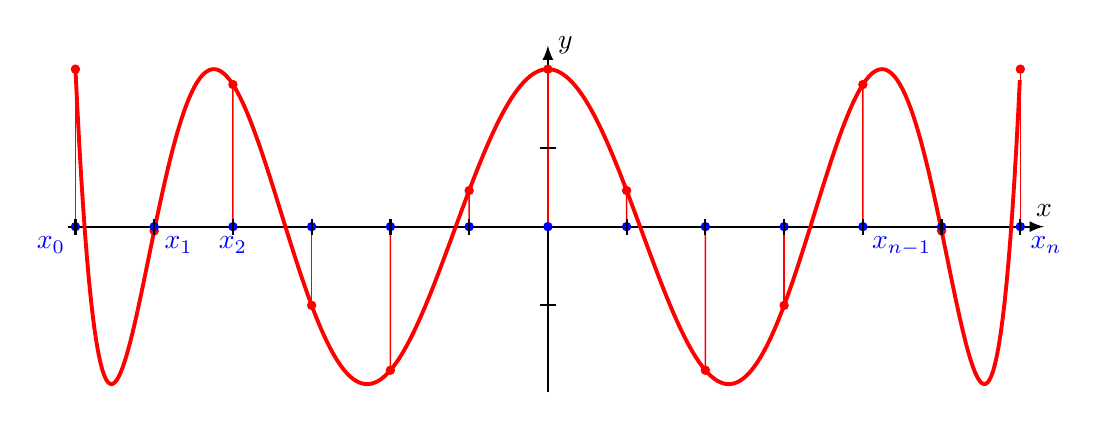
\begin{tikzpicture}[>=latex,thick]

\draw[->] (-6.1,0)--(6.3,0) coordinate[label={$x$}];
\draw[->] (0,-2.1)--(0,2.3) coordinate[label={right:$y$}];

\uncover<6->{%
\draw[color=red,line width=1.4pt]
	plot[domain=-1:1,samples=500]
		({6*\x},{2*((((128*\x*\x-256)*\x*\x+160)*\x*\x-32)*\x*\x+1)});
}

\uncover<2->{%
\node[color=blue] at (-6,0) [below left] {$x_0$};
\node[color=blue] at (-5,0) [below right] {$x_1$};
\node[color=blue] at (-4,0) [below] {$x_2$};
\node[color=blue] at (5,0) [below left] {$x_{n-1}$};
\node[color=blue] at (6,0) [below right] {$x_{n}$};
\foreach \y in {-6,-5,...,6}{
	\pgfmathparse{\y/6}
	\xdef\x{\pgfmathresult}
	\uncover<4->{
	\draw[color=red,line width=0.5pt]
		(\y,0)--
		({6*\x},{2*((((128*\x*\x-256)*\x*\x+160)*\x*\x-32)*\x*\x+1)});
	\fill[color=red]
		({6*\x},{2*((((128*\x*\x-256)*\x*\x+160)*\x*\x-32)*\x*\x+1)})
			circle[radius=0.06];
	}
	\fill[color=blue]
		({6*\x},0) circle[radius=0.06];
}}

\foreach \x in {1,...,6}{
	\draw (\x,-0.1)--(\x,0.1);
	\draw (-\x,-0.1)--(-\x,0.1);
}
\draw (-0.1,-1)--(0.1,-1);
\draw (-0.1,1)--(0.1,1);

\end{tikzpicture}}
\end{center}
\end{frame}
